\chapter{Matematik}
%%
%%
\section{Polære Koordinater, Cosinus og Sinus}
%%
%%
\begin{opgave}{Idiotformlen}{1}
Brug at $\cos \theta$ og $\sin \theta$ er hhv. den hosliggende og modstående katete i en retvinklet trekant med hypotenuse 1 pr. deres definition. Tegn det i enhedscirklen. Det giver da, at $\cos^2 (\theta) + \sin^2 (\theta) = 1^2 = 1$ fra Pythagoras sætning. 
\end{opgave}
%%
%%
\begin{opgave}{Tangens}{1}
Fra definitionen af tangens har vi, at $\tan(\theta) = \sin(\theta)/\cos(\theta)$. Men i matematikafsnittet er det også introduceret, at $\cos(\theta)$ er givet som længden af den hosliggende katete divideret med længden af hypotenusen, og at $\sin(\theta)$ er givet som længden af den modstående katete divideret med længden af hypotenusen. 
\begin{align*}
gg
\end{align*}
\end{opgave}
\section*{Differentialregning}
\begin{opgave}{Afledte og dobbeltafledte}{1}
\opg $f(x) = x^3$: 
\begin{equation*}
\dif{x}{f}=3x^2,~~ \dif[2]{x}{f}=6x
\end{equation*}
\opg $f(x) = x^2 + 4x$:
\begin{equation*}
\dif{x}{f}=2x+4,~~ \dif[2]{x}{f}=2
\end{equation*}
\opg $f(x) = \frac{1}{x} + \frac{1}{x^2}=x^{-1}+x^{-2}$: 
\begin{equation*}
\dif{x}{f} = - x^{-2}-2x^{-3}, ~~\dif[2]{x}{f}=2x^{-3}+6x^{-4}
\end{equation*}
\opg $f(x) = \cos (x)$: 
\begin{equation*}
\dif{x}{f}= - \sin (x),~~ \dif[2]{x}{f}=-\cos (x)
\end{equation*}
\opg $f(x) = \ln (x)$: 
\begin{equation*}
\dif{x}{f}= \frac{1}{x}=x^{-1},~~\dif[2]{x}{f}=-x^{-2}
\end{equation*}
\end{opgave}

\begin{opgave}{Ubestemte integraler}{1}
\opg $f(x) = x^3$: 
\begin{equation*}
\int f(x) \d x = \frac{1}{4}x^4 +C
\end{equation*}
\opg $f(x) = x^2 + 4x$:
\begin{equation*}
\int f(x) \d x = \frac{1}{3}x^3 + 2x^2 + C
\end{equation*}
\opg $f(x) = \frac{1}{x} + \frac{1}{x^2}=x^{-1}+x^{-2}$: 
\begin{equation*}
\int f(x) \d x = \ln (x) -x^{-1} + C
\end{equation*}
\opg $f(x) = \cos (x)$: 
\begin{equation*}
\int f(x) \d x = \sin(x)+C
\end{equation*}
\opg $f(x) = \ln (x)$: 
\begin{equation*}
\int f(x) \d x = x\ln (x) -x + C
\end{equation*}
\end{opgave}

\begin{opgave}{Sammensatte funktioner}{1}
$g(x)$ og $f(g)$ findes. $\dif{x}{f}$ findes vha. kædereglen: $\dif{x}{f} = \dif{x}{g} \cdot \dif{g}{f}$.
\opg $f(x) = \sin (4x)$:
\begin{align*}
g(x) &= 4x, ~~f(g)=\sin(g) \\
\rightarrow &\dif{x}{f} = 4\cos(4x)
\end{align*}
\opg $f(x) = \sqrt{2x}$:
\begin{align*}
g(x) = 2x, ~~ f(g)=\sqrt{g} \\
\rightarrow \dif{x}{f} = 2\frac{1}{2\sqrt{2x}}=\frac{1}{\sqrt{2x}}
\end{align*}
\opg $f(x) = \sqrt{4x+5}$
\begin{align*}
g(x) = 4x+5, ~~f(g)=\sqrt{g} \\
\rightarrow \dif{x}{f} = 4\frac{1}{2\sqrt{4x+5}}=\frac{2}{\sqrt{4x+5}}
\end{align*}
\opg $f(x) = \sin(e^x)$
\begin{align*}
g(x) = e^x, ~~f(g)=\sin(g) \\
\rightarrow \dif{x}{f} = e^x \cos(e^x)
\end{align*}
\end{opgave}

\begin{opgave}{Integration ved substitution}{1}
Udregn de følgende integraler vha. integration ved substitution:
\opg $\int e^{-4x} \d x$
\begin{align*}
\int e^{-4x} \d x = -\frac{1}{4}e^{-4x} + C
\end{align*}
\opg $\int \sqrt{3x-2} \d x$
\begin{align*}
\int \sqrt{3x-2} \d x = \frac{2}{9}\cdot(3x-2)^{\frac{3}{2}} + C
\end{align*}
\opg $\int xe^{-3x^2} \d x$
\begin{align*}
\int xe^{-3x^2} \d x = -\frac{1}{6}e^{-3x^2}+C
\end{align*}
\opg $\int \frac{x-1}{\sqrt{x+1}} \d x$
\begin{align*}
\int \frac{x-1}{\sqrt{x+1}} \d x = \frac{2}{3}\sqrt{x+1}(x-5)
\end{align*}
\end{opgave}

\begin{opgave}{$\boldsymbol{f}$ som funktion af $\boldsymbol{g}$}{1}
Udtryk $\d{f}{x}$ vha. den ukendte funktion $g(x)$ og dens
differentierede $\dif{x}{g}$ for følgende funktioner:
\opg $f(x) = x^2 g(x)$. Produktreglen anvendes:
\begin{equation*}
\dif{x}{f} = \dif{x}{x^2}\cdot g(x) + x^2\dif{x}{g} = 2xg(x)+x^2 \dif{x}{g}
\end{equation*}
\opg $f(x) = \left(g(x)\right)^2$. Produktreglen anvendes:
\begin{equation*}
\dif{x}{f} = \dif{x}{g} g(x) + g(x)\dif{x}{g} = 2g(x)\dif{x}{g}
\end{equation*}
\opg $f(x) = g(x^2)$. Kædereglen anvendes:
\begin{equation*}
\d{f}{x}=2x\d{g}{x^2}
\end{equation*}
\end{opgave}

\begin{opgave}{Partiel integration}{2}
Udregn de følgende integrale vha. partiel integration og substitution:
\opg $\int 4x\cos(2-3x)\d x$
\begin{align*}
	\int 4x\cos(2-3x)\d x = \frac{4}{9}\cos(2-3x)-\frac{4}{3}x\sin(2-3x) +C
\end{align*}
\opg $\int (2+5x)e^{\frac{1}{3}x}\d x$
\begin{align*}
	\int (2+5x)e^{\frac{1}{3}x}\d x = (15x-39)e^{\frac{1}{3}x}+C
\end{align*}
\opg $\int (3x+x^2)\sin (2x) \d x$
\begin{align*}
	\int (3x+x^2)\sin (2x) \d x = -\frac{1}{2}(3x+x^2)\cos (2x) +\frac{1}{4}\Big[ (3+2x)\sin (2x) + \cos (2x) \Big] + C
\end{align*}
\end{opgave}

\begin{opgave}{Hastighed og postion}{1}
\begin{figure}[h!]
  \centering
%  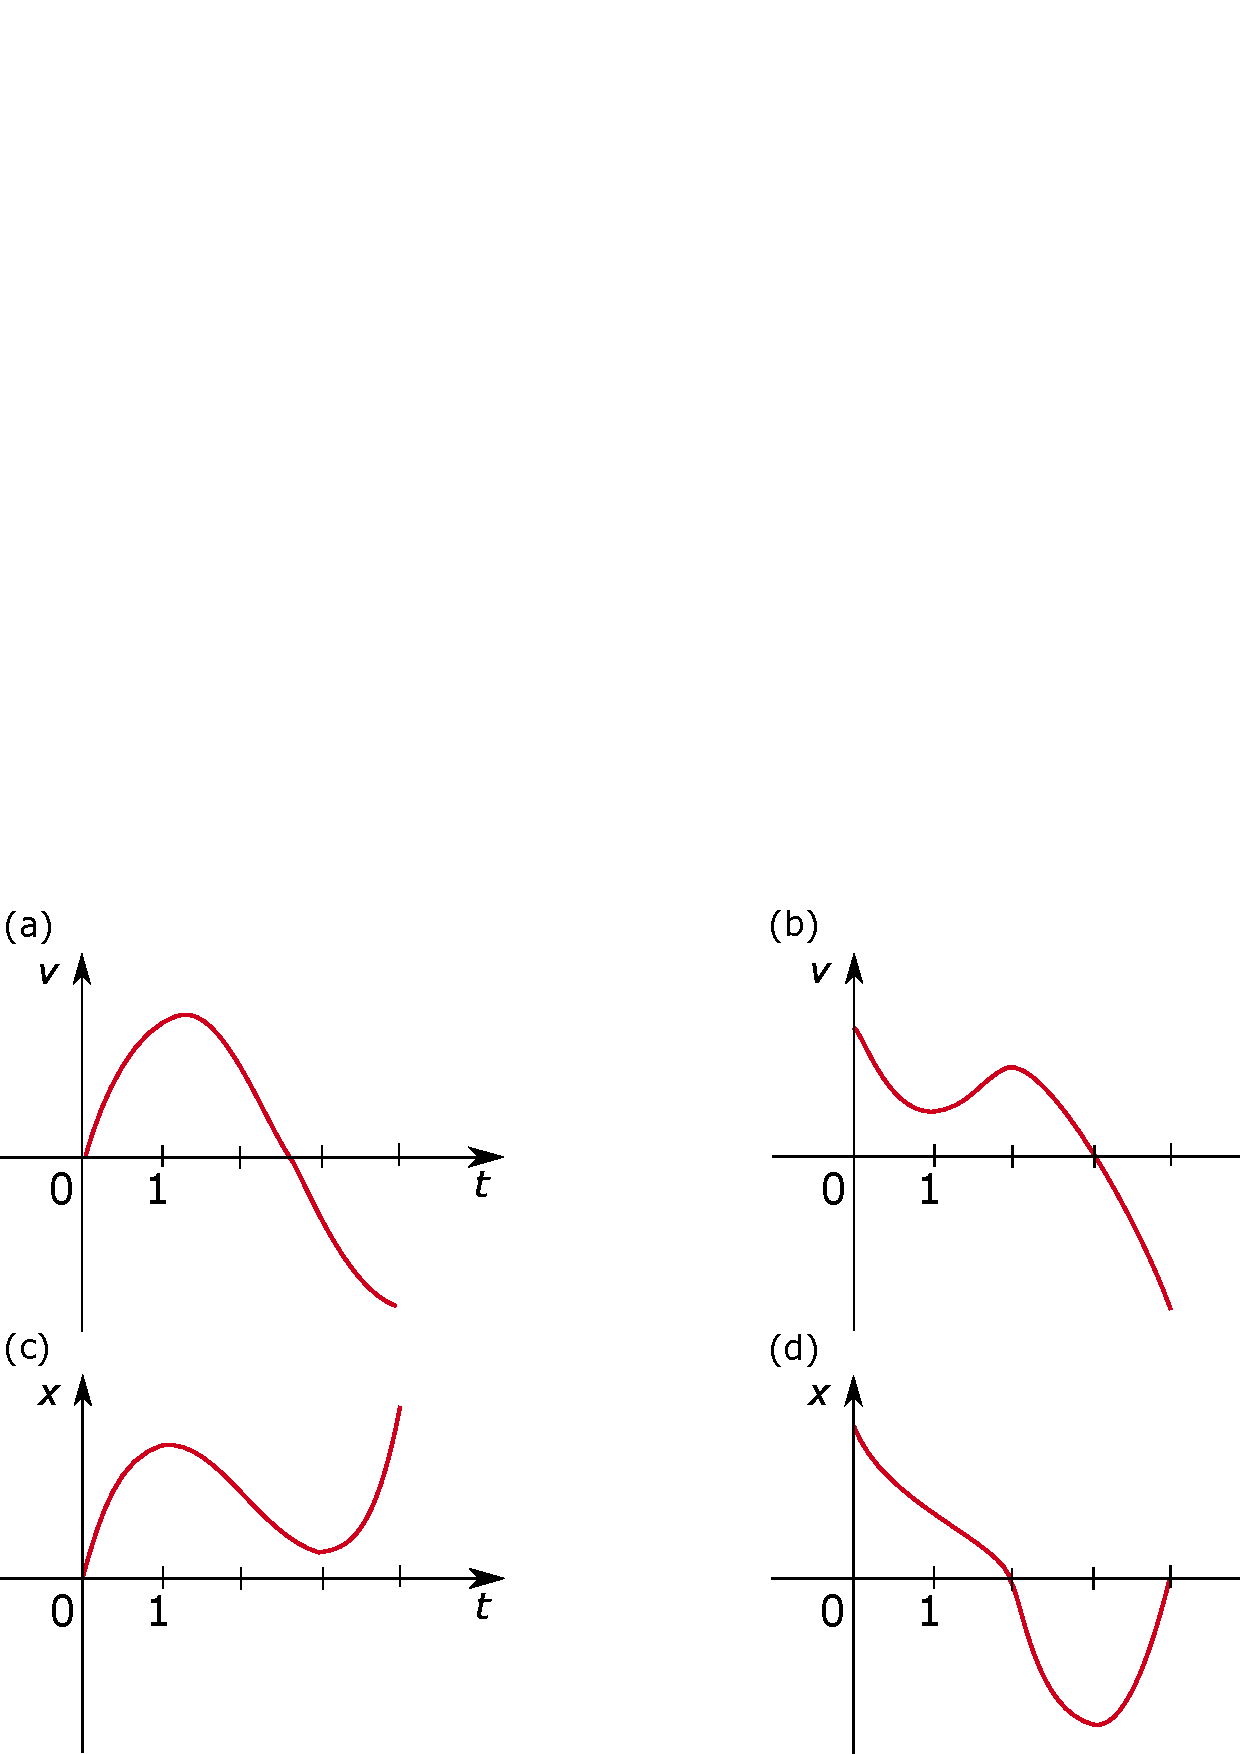
\includegraphics[width=0.6\textwidth]{matematik/vx_grafer.png}
  \caption{Hastighed og position som funktion af tiden.}
  \label{fig:vx_grafer}
\end{figure}
\opg Da grafen simpelt viser $v$ som funktion af tiden kan man bare aflæse på figuren.
for (a): 
\begin{itemize}
\item $t= 0 \rightarrow 1,5$: sætter farten op
\item $t= 1,5 \rightarrow 4$: sætter farten ned
\end{itemize}
for (b):
\begin{itemize}
\item $t= 0 \rightarrow 1$: sætter farten ned
\item $t= 1 \rightarrow 2$: sætter farten op
\item $t= 2 \rightarrow 4$: sætter farten ned
\end{itemize}
.
\opg Her ses i stedet positionen som funktion af tiden. For at svare på, hvordan hastigheden opfører sig, så skal vi derfor kigge på \emph{hældningen} af grafen.
for (c): 
\begin{itemize}
\item $t= 0 \rightarrow 1$: positiv hældning $\rightarrow$ hastigheden øges
\item $t= 1 \rightarrow 3$: negativ hældning $\rightarrow$ hastigheden sænkes
\item $t= 3 \rightarrow 4$: positiv hældning $\rightarrow$ hastigheden øges
\end{itemize}
for (d):
\begin{itemize}
\item $t= 0 \rightarrow 2$: negativ hældning $\rightarrow$ hastigheden sænkes
\item $t= 2 \rightarrow 3$: negativ hældning $\rightarrow$ hastigheden sænkes - og hældningen er større, så der bremses hårdere.
\item $t= 3 \rightarrow 4$: positiv hældning $\rightarrow$ hastigheden øges
\end{itemize}
.
\end{opgave}
\begin{opgave}{Harmonisk bevægelse}{2}
\begin{equation*}
x = A \cos (\omega t + \phi),
\end{equation*}
hvor $A$, $\omega$ og $\phi$ er konstanter. 
\opg For at finde hastigheden ($\dt{x}$), så ses det at udtrykket er en sammensat funktion ($g=\omega t+\phi$, $f=A\cos g$). Bruges kædereglen får man:
\begin{equation*}
\dt{x} = - A\omega \sin(\omega t + \phi)
\end{equation*}
\opg Hvis det antages at alle konstanter er $>0$, så er $\dt{x}=0$, når $\sin(\omega t + \phi) = 0$. Det er opfyldt for $\omega t + \phi = 0, \pi, 2\pi, ...$. Fysisk set er $v=0$ i yderpunkterne af svingningen, som forekommer periodisk.
\end{opgave}
\begin{opgave}{Cepheide-stjernen Delta Cephei}{2}
\begin{equation*}
B(t) = 4,0 + 0,35\sin \left( \frac{2\pi t}{5,4} \right).
\end{equation*}
\opg Raten er $\dif{t}{B} = \dt{B}$. Funktionen er en sammensat funktion ($u=\frac{2\pi t}{5,4}, g=0,4+0,35 \sin u$).
\begin{equation*}
\dt{B} = 0,35 \cdot \frac{2\pi}{5,4} \cos \left( \frac{2\pi t}{5,4} \right)
\end{equation*}
\opg For at finde ændringen i lysstyrke udregnes forskellen:
\begin{align*}
B(t=\text{2 dage})-B(t=\text{0 dage}) \\
&= 4,0 + 0,35\sin\left(\frac{2\pi}{5,4} \cdot 2 \right) - 4,0 -0,35\sin\left(\frac{2\pi}{5,4} \cdot 0 \right) \\
&= 0,25
\end{align*}
Husk at regne i radianer og ikke i grader.
\end{opgave}

\begin{opgave}{Udvidelse af ballon}{2}
\opg $\dif{r}{V}$ er ændring af volumen afhængig af radius, mens $\dif{t}{V}$ er ændring af volumen afhængig af tiden.
\opg Volumenet af en sfærisk ballon er $V(t)=\frac{4}{3} \pi r(t)^3$. Det er en sammensat funktion med $u=r(t)$ og $g=\frac{4}{3} \pi u^3$. Det giver:
\begin{equation*}
\dt{V} = \frac{4}{3} 2\pi \cdot 3 r^2(t) \dt{r}
\end{equation*}
\end{opgave}

\begin{opgave}{Approksimation af funktion}{3}
  \[
  f(x) = f(a) + (x-a) \left.\d{f}{x}\right|_{x=a}
  + \frac{1}{2} (x-a)^2 \left.\dif[2]{x}{f}\right|_{x=a}
  + \frac{1}{3!} (x-a)^3 \left.\dif[3]{x}f\right|_{x=a}
  + \ldots
  \]
  \opg Første led er en konstant, mens andet led afhænger linært af $x$, og tredje led kvadratisk af $x$ osv. Forfaktoren bliver mindre og mindre for hvert led, så ledene bliver mindre og mindre.
  \opg For $x \approx 0$, er $\sin (x)$ med de første to led:
  \begin{align*}
  \sin x &= \sin(0) + (x-0) \left. \dif{x}{\sin (x)}\right|_{x=0} \\
  &= 0 + x\cos(0) \\
  &= x
  \end{align*}
  Idet $\sin(0)=0$ og $\cos(0)=1$.
  For $x \approx 0$, er $\cos x$ med de første to led:
  \begin{align*}
  \cos (x) &= \cos(0) + (x-0) \left.\dif{x}{\sin (x)}\right|_{x=0} \\
  &= 1 -x\sin(0) \\
  &= 1
  \end{align*}
  Hvis man medtager det 3. led, så bliver $\sin(x)$:
  \begin{align*}
  \sin(x) &= x + \frac{1}{2} (x-0)^2 \left. \dif[2]{x}{\sin(x)}\right|_{x=0} \\
  &= x - \frac{x^2}{2} \sin(0) \\
  &= x  
  \end{align*}
  Hvis man medtager det 3. led, så bliver $\cos(x)$:
  \begin{align*}
  \cos(x) &= 1 + \frac{1}{2} (x-0)^2 \left.\dif[2]{x}{\cos(x)}\right|_{x=0} \\
  &= 1 - \frac{x^2}{2} \cos(0) \\
  &= 1 - \frac{x^2}{2}  
  \end{align*}
  \opg For $x \approx 1$, er $\ln (x)$ for de tre første to led:
  \begin{align*}
  \ln x &= \ln(1) + (x-1) \left. \dif{x}{\ln (x)} \right|_{x=1} + \frac{1}{2} \left(x-1\right)^2 \left. \dif[2]{x}{\ln (x)}\right|_{x=1} \\
  &= 0 + (x-1)\frac{1}{1} - \frac{1}{2} \left( x^2 +1 - 2x \right) \left. \dif{x}{} \frac{1}{x} \right|_{x=1} \\
  &= x -1 + \frac{1}{2} \left( x^2 + 1 - 2x \right) \left. \left( -1 x^{-2} \right)\right|_{x=1} \\
  &= x - 1 - \frac{x^2}{2} - \frac{1}{2} + x\\
  &= - \frac{x^2}{2} + 2x - \frac{3}{2}
  \end{align*}
  Idet den differentierede at $\ln (x) = \frac{1}{x}$ og $\ln (1)=0$.
  \opg For $x \approx 0$, er $e^x \approx 1 + x + \frac{1}{2}
  x^2$ for de første tre led:
  \begin{align*}
  e^x &= e^0 + (x-0) \left. \dif{x}{e^x}\right|_{x=0} + \frac{1}{2}(x-0)^2 \left. \dif[2]{x}{e^x}\right|_{x=0} \\
  &=1 + x + \frac{1}{2} x^2,
  \end{align*}
  Idet den differentierede af $e^x$ er $e^x$ og $e^0 = 1$.
  \opg For $x \approx 0$, vises det, at approksimationen for et polynomie
  $a_0 + a_1 x + a_2 x^2 + \ldots$ er givet ved leddene i polynomiet
  selv. Vi regner ét led af gangen:
  \begin{align*}
  \text{Første led } &= a_0 + a_1\cdot 0 + a_2 \cdot 0^2 \\
  &= a_0 \\
  \text{Andet led } &= (x-0) \left. \dif{x}{} \left(a_0 + a_1x + a_2x^2 \right)\right|_{x=0} \\
  &= x \cdot \left. \left(a_1 + 2a_2x) \right)\right|_{x=0} \\
  &= a_1 x \\
  \text{Tredje led} &= \frac{1}{2} \left( x-0 \right)^2 \left. \dif[2]{x}{} \left(a_0 + a_1x + a_2x^2 \right)\right|_{x=0} \\
  &= \frac{1}{2} x^2 \left. \dif{x}{} \left(a_1 + 2a_2x \right)\right|_{x=0} \\
  &= \frac{1}{2} x^2 \left. \left( 2a_2 \right)\right|_{x=0} \\
  &= a_2 x^2 \\
  \rightarrow & a_0 + a_1x+a_2x^2
  \end{align*}
  Og det er hermed vist at approksimationen af et polynomie er givet ved leddene i polynomiet.
  \opg For små værdier af $x$ ($x \approx 0$), vises det, at $(1 + x)^a \approx 1 + ax$.:
  \begin{align*}
  (1+x)^a &= (1+0)^a + (x-0) \left. \dif{x}{(1+x)^a}\right|_{x=0} \\
  &= 1 + \left. \left( a(1+x)^{a-1} \right)\right|_{x=0} \\
  &= 1 + ax,
  \end{align*}
  hvor $(1+x)^a$ er blevet differentieret som en sammensat funktion med $u=1+x$ og $g=u^a$.
\end{opgave}

\begin{figure}
	\centering
%	\includegraphics[width=\columnwidth]{/matematik/fig/JordensForm.pdf}
	\caption{Plot af $f(x),g(x)$, samt approksimationer af disse.} \label{fig:JordensForm}
\end{figure}
\begin{opgave}{Jordens form}{2}
I første omgang differentieres funktionen to gange vha. kædereglen
\begin{align*}
	\dif{x}{f(x)} &= \frac{1}{2}\left[R^2 - x^2\right]^{-1/2}(-2x) \\
	&= \frac{-x}{\sqrt{R^2 - x^2}} \\
	\dif[2]{x}{f(x)} &= \dif{x}{}\left(\frac{-x}{\sqrt{R^2 - x^2}}\right) \\
	&= -\frac{1}{2}\left[R^2 - x^2\right]^{-3/2}(-x)(-2x) - \left[R^2 - x^2\right]^{-1/2} \\
	&= \frac{-x^2}{(R^2 - x^2)^{3/2}} - \frac{1}{\sqrt{R^2 - x^2}}
\end{align*}
Evalueres disse differentialer i $x = 0$ fås
\begin{align*}
	\left.\dif{x}{f(x)}\right|_{x=0} &= \left[\frac{-x}{\sqrt{R^2 - x^2}}\right]_{x=0} \\
	&= \frac{-0}{\sqrt{R^2 - 0^2}} \\
	&= 0 \\
	\left.\dif[2]{x}{f(x)}\right|_{x=0} &= \left[\frac{-x^2}{(R^2 - x^2)^{3/2}} - \frac{1}{\sqrt{R^2 - x^2}}\right]_{x=0} \\
	&= \frac{-0^2}{(R^2 - 0^2)^{3/2}} - \frac{1}{\sqrt{R^2 - 0^2}} \\
	&= 0 - \frac{1}{R} \\
	&= -\frac{1}{R}
\end{align*}
\opg Indsættes det i ligning \ref{k-Taylor_pol} fra kompendiet fås
\begin{align*}
	f_2(x) &\simeq f(0) + x\left.\dif{x}{f(x)}\right|_{x=0} + \frac{1}{2}x^2\left.\dif[2]{x}{f(x)}\right|_{x=0} \\
	&= R + 0 - \frac{1}{R}x^2
\end{align*}
hvilket er Taylorrækken til 2. orden. Til første og nulte orden er det
\begin{align*}
	f_1(x) &\simeq R + 0 = R \\
	f_0(x) &\simeq R
\end{align*}
\opg Da $f_0(x) = f_1(x)$ betragtes de herfra sammen. \\
1) \enspace $f_1$ er en vandret linje for alle værdier af $x$ \\
2) \enspace $f_2(x)$ er en parabel, hvor "benene" vender nedad, grundet fortegnet på højesteordensledet.
\opg Se figur \ref{fig:JordensForm}.
\opg Der er tale om \\
1) \enspace Et plan. \\
2) \enspace En elliptisk paraboloid, dvs. den figur, der fremkommer ved at dreje en parabel\SI{180}{\degree} rundt om $y$-aksen. Af denne figur er taget de positive værdier og spejlet i $x$-aksen. Denne forklaring giver ikke super meget mening, hvorfor det er bedre bare at tænke det som et øje.
\opg På bagrund af dette er det acceptable approksimationer at se jorden som enten flad eller et gigantsisk øje. Som figuren dog viser er det begrænset, hvor stort et område disse approksimationer er valide.
\end{opgave}

\newpage

\section*{Differentialligninger}

\begin{opgave}{Specialtilfælde af 1. og 2. Ordens Differentialligninger}{1}
\opg $f(t) = -7e^{3t}$ og $\dif{t}{f} = 3f(t)$.

$$\dif{t}{f} = -7 \dif{t}{} e^{3t} = -7 \cdot 3 e^{3t} = 3 \left( -7 e^{3t} \right) = 3 f(t)$$
\vspace{2mm}
\opg $g(t) = \frac{2}{3}e^t + e^{-2t}$ og $\dif{t}{g} + 2g(t) = 2e^t$.

$$\dif{t}{g} = \frac{2}{3} \dif{t}{}e^t + \dif{t}{} e^{-2t} = \frac{2}{3}e^t -2e^{-2t} \quad \Rightarrow \quad \dif{t}{g} + 2g(t) = \frac{2}{3}e^t -2e^{-2t} + \frac{4}{3}e^t + 2e^{-2t} = \frac{6}{3} e^t = 2e^t$$
\vspace{2mm}
\opg $h(t) = 5 \sin(3t) - 10\cos(3t)$ og $\dif[2]{t}{h} = -9h(t)$.

$$\dif{t}{h} = 3 \cdot 5 \cos(3t) + 3 \cdot 10 \sin(3t) \quad \Rightarrow \quad \dif[2]{t}{h} = (-9) \cdot 5 \cos(3t) + 9 \cdot 10 \sin(3t) = -9 h(t)$$
\vspace{2mm}
\opg $k(t) = 13 \cos \left( 8t + 45 \right)$ og $\dif[2]{t}{k} = -64 k(t)$.

$$\dif{t}{k} = (-8) \cdot 13 \cos \left( 8t + 45 \right) \quad \Rightarrow \quad \dif[2]{t}{k} = (-64) \cdot 13 \cos \left( 8t + 45 \right) = -64 k(t)$$
\vspace{2mm}
\end{opgave}

\begin{opgave}{Generelle 1. Ordens Differentialligninger}{2}
\opg $h(x) = 1/ \left( x+A \right)$ og $\dif{x}{h} = -h(x)^2$.

$$\dif{x}{f} = \dif{x}{}\left( x+A \right)^{-1} = - \left( x+A \right)^{-2} \dif{x}{}\left( x+A \right) = - \frac{1}{\left( x + A \right)^2} = -h(x)^2$$
\vspace{2mm}
\opg $k(x) = \left( c-x^2 \right)^{-1/2}$ og $\d{k}{x} = x k(x)^3$.

$$\dif{x}{k} = - \frac{1}{2} \left( c-x^2 \right)^{-3/2}  \dif{x}{}\left( c-x^2 \right) = x \left( c-x^2 \right)^{-3/2} = x k(x)^3$$
\vspace{2mm}
\opg $g(x) = \left( \ln (x) + C \right)/x$ og $x^2 \dif{x}{g} + x g(x) = 1$.

\begin{align*}
	\dif{x}{g} &= \left[ \dif{x}{}\left( \ln x + C \right) \right] \frac{1}{x} + \left( \ln x + C \right)  \left[ \dif{x}{}\frac{1}{x} \right]  = \frac{1}{x^2} - \frac{\ln x + C}{x^2} \\ &\Rightarrow x^2 \dif{x}{g} + xg(x) = 1 - \left( \ln (x) + C \right) + \left( \ln (x) + C \right) = 1
\end{align*}
\vspace{2mm}
\opg $f(x) = \left( 1+ce^x \right)/\left( 1-ce^x \right)$ og $\dif{x}{f} = \frac{1}{2} \left( f(x)^2 -1 \right)$.

\begin{align*}
\dif{x}{f} &= \left[ \dif{x}{}\left( 1+c^x \right) \right] \frac{1}{1-ce^x} + \left( 1+ce^x \right) \left[ \dif{x}{}\frac{1}{1-ce^x} \right] = \frac{ce^x}{1-ce^x} +  \frac{\left( 1+ce^x \right) \left( -1 \right) \left( -ce^x \right)}{\left( 1-ce^x \right)^2}\\\\
&= ce^x \left[ \frac{1}{1-ce^x} + \frac{1+ce^x}{\left( 1-ce^x \right)^2} \right] = ce^x \frac{1-ce^x + 1+ce^x}{\left( 1-ce^x \right)^2} = \frac{2ce^x}{\left( 1-ce^x \right)^2}
\end{align*}

\begin{align*}
	f(x)^2 - 1  &=  \frac{\left( 1+ce^x \right)^2}{\left( 1-ce^x \right)^2} - \frac{(1-ce^x)^2}{\left( 1-ce^x \right)^2} = \frac{\left( 1+ce^x \right)^2 - \left( 1-ce^x \right)^2}{\left( 1-ce^x \right)^2} = \frac{4ce^x}{\left( 1-ce^x \right)^2} \\
	&\Rightarrow \dif{x}{f} = \frac{1}{2} \left( f(x)^2 -1 \right)
\end{align*}
\end{opgave}

\begin{opgave}{Hvornår er det en løsning?}{3}
\opg Find $k$ så $f(y) = \cos(ky)$ løser $4 \dif[2]{y}{f} = -25f(y)$.

$$\dif{y}{f} = -k\sin(ky) \quad \Rightarrow \quad \dif[2]{y}{f} = -k^2 \cos(ky) = -k^2 f(y)$$

\vspace{2mm}

Så sætter man ind:

$$4 \dif[2]{y}{f} = -25f(y) \quad \Rightarrow \quad -4k^2 f(y) = -25f(y) \quad \Rightarrow \quad k^2 = \frac{25}{4} \quad \Rightarrow \quad k = \pm \frac{5}{2}$$
\vspace{2mm}
\opg For de fundne $k$ fra 1), vis at $g(y) = A\sin(ky) + B\cos(ky)$ løser $4 \dif[2]{y}{g} = -25g(y)$.

$$\dif{y}{g} = kA\cos(ky) - kB\sin(ky) \quad \Rightarrow \quad \dif[2]{y}{g} = -k^2 A \sin(ky) - k^2 B \cos(ky) = -k^2g(y)$$

\vspace{2mm}

Det giver:

$$-4k^2 g(y) = -25g(y) $$

\vspace{2mm}

Som er opfyldt for $k = \pm \frac{5}{2}$.\\
\opg Find $r$ så $h(y) = e^{ry}$ løser $2 \dif[2]{y}{h} + \dif{y}{h} - h(y) = 0$.

$$\dif{y}{h} = re^{ry} = rh(y) \quad \Rightarrow \quad \dif[2]{y}{h} = r^2 e^{ry} = r^2 h(y)$$

\vspace{2mm}

Så sætter man ind:

$$2 \dif[2]{y}{h} + \dif{y}{h} - h(y) = 0 \quad \Rightarrow \quad 2r^2h(y) + rh(y) -h(y) = 0 \quad \Rightarrow \quad 2r^2+r-1=0$$
\vspace{2mm}

Løses andengradsligningen får man:

$$r_1 = \frac{1}{2} \quad \text{og} \quad r_2 = -1$$ 
\vspace{2mm}
\opg For de fundne $r_1,r_2$ i 3), vis at $k(y) = ae^{r_1y} + be^{r_2y}$ løser $2 \dif[2]{y}{k} + \dif{y}{k} - k(y) = 0$.

$$\dif{y}{k} = ar_1e^{r_1y} + br_2e^{r_2y} \quad \Rightarrow \quad \dif[2]{y}{k} = ar_1^2e^{r_1y} + br_2^2e^{r_2y}$$ 
\vspace{2mm}

Så sætter man ind:

\begin{align*}
2 \dif[2]{y}{k} + \dif{y}{k} - k(y) &= 2 \left( ar_1^2e^{r_1y} + br_2^2e^{r_2y}  \right) + \left( ar_1e^{r_1y} + br_2e^{r_2y} \right) - \left( ae^{r_1y} + be^{r_2y} \right)\\\\ 
&= \left( 2ar_1^2 + ar_1 - a \right)e^{r_1y} + \left( 2br_2^2 + br_2 - b \right)e^{r_2y} = 0 \cdot e^{r_1y} + 0 \cdot e^{r_2y} = 0 
\end{align*}
\end{opgave}